\documentclass{article}

\usepackage{graphicx}
\usepackage{tikz}
\usepackage{tikzsymbols}
\usetikzlibrary{calc,patterns,shapes.geometric}
\pagestyle{empty}
\usepackage[margin=0pt]{geometry}
\geometry{papersize={14in,12in}}

\def\centerarc[#1](#2)(#3:#4:#5){\draw[#1] ($(#2)+({#5*cos(#3)},{#5*sin(#3)})$) arc (#3:#4:#5);}

\begin{document}
	\begin{figure}
		\centering
		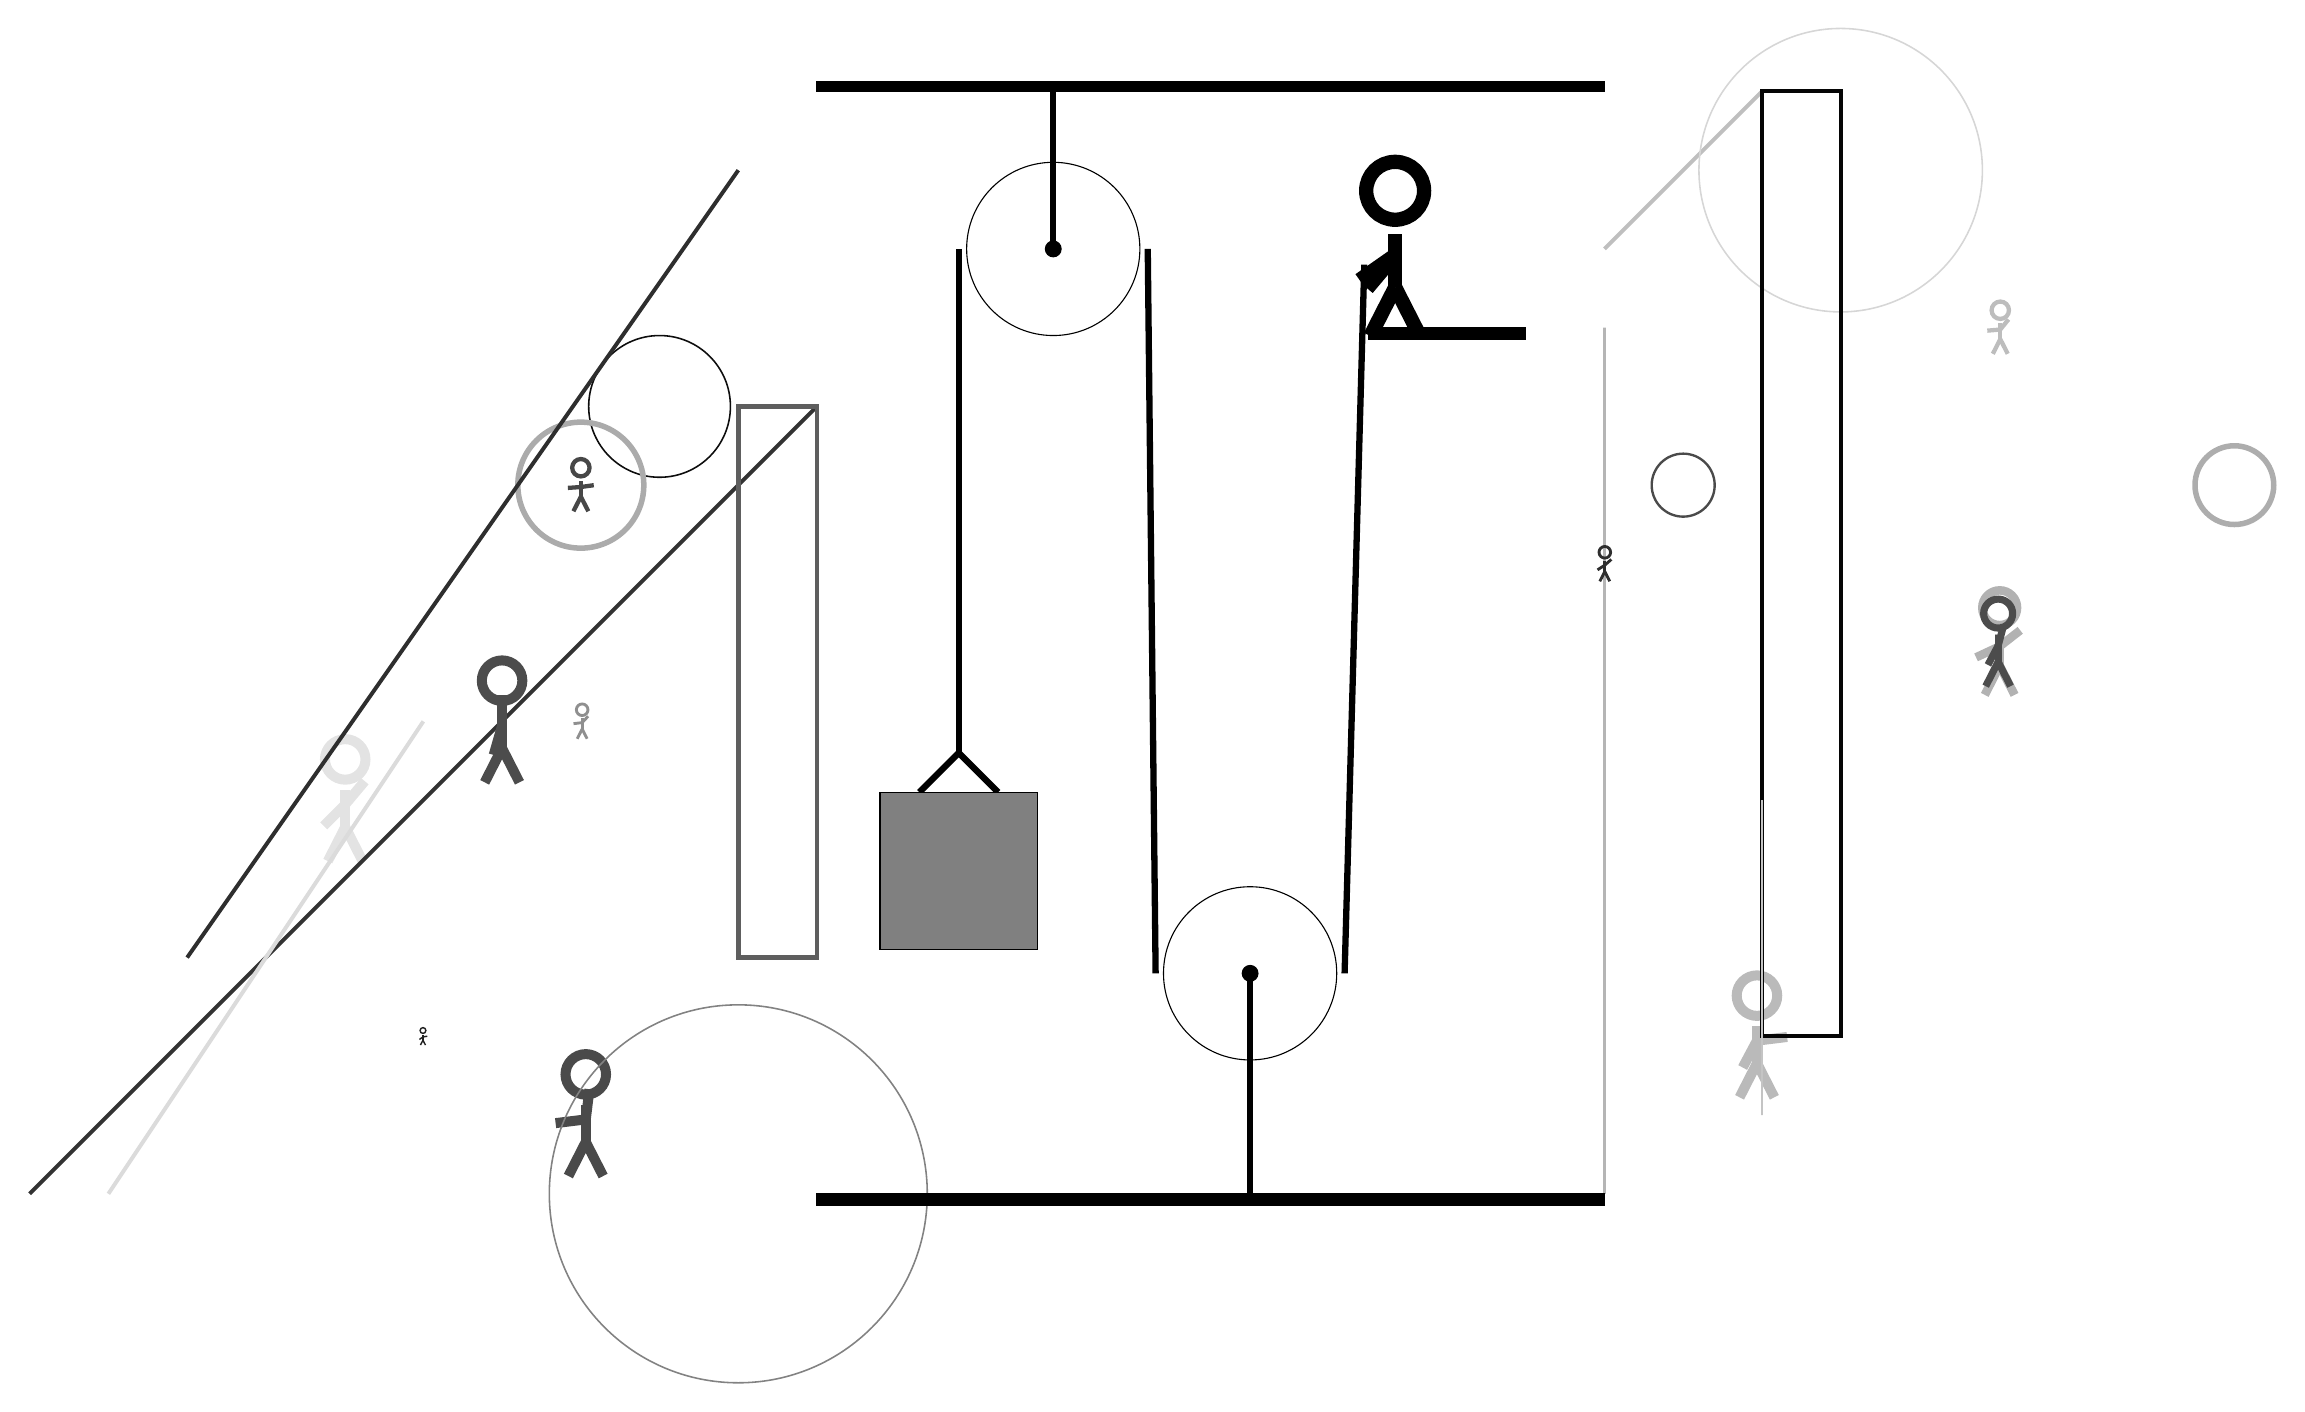
\begin{tikzpicture}
			%%%%% START %%%%%
			
			\draw[fill=black] (-2, 14) rectangle (8, 14.125);
			
			\draw (3.5, 2.8) circle (1.1);
			\draw[fill=black] (3.5, 2.8) circle (0.1);
			\draw[line width=0.8mm] (3.5, 2.8) -- (3.5, 0);
			
			\draw (1, 12) circle (1.1);
			\draw[fill=black] (1, 12) circle (0.1);
			\draw[line width=0.8mm] (1, 14) -- (1, 12);
			
			\draw[line width=0.8mm](-0.7, 5.1) --  (-0.2, 5.6) -- (0.3, 5.1);
			\draw[fill=black!50] (-1.2, 5.1) rectangle (0.8, 3.1);
			
			\draw[line width=0.8mm](-0.2, 12) -- (-0.2, 5.6);
			\centerarc[line width=0.8mm](1, 12)(180:0:1.2000000000000002)
			\draw[line width=0.8mm](2.2, 12) -- (2.3, 2.8);
			\centerarc[line width=0.8mm](3.5, 2.8)(180:360:1.2000000000000002)
			\draw[line width=0.8mm](4.7, 2.8) -- (4.95, 11.8);
			
			\node at (5.3, 12) {\Strichmaxerl[10][35][-130]};
			\draw[fill=black] (5, 11) rectangle (7, 10.85);
			
			\node[line width=0.3mm, color=black!71] at (-5, 1) {\Strichmaxerl[7][7][83]};
			
			\draw [line width=0.2mm, color=black!95](-4, 10) circle (0.9);
			\draw[line width=0.3mm, color=black!29] (8, 11) rectangle (8, 0);
			\node[line width=0.7mm, color=black!11] at (-8, 5) {\Strichmaxerl[7][45][50]};
			
			\node[line width=0.5mm, color=black!87] at (-7, 2) {\Strichmaxerl[1][35][10]};
			
			\draw[line width=0.5mm, color=black!25](10, 14) -- (8, 12);
			\draw [line width=0.7mm, color=black!32](16, 9) circle (0.5);
			\draw[line width=0.5mm, color=black!80](-2, 10) -- (-12, 0);
			\node[line width=0.2mm, color=black!72] at (-5, 9) {\Strichmaxerl[3][4][8]};
			\draw [line width=0.2mm, color=black!16](11, 13) circle (1.8);
			
			\draw[line width=0.5mm, color=black!14](-7, 6) -- (-11, 0);
			\node[line width=0.6mm, color=black!27] at (10, 2) {\Strichmaxerl[7][62][7]};
			\draw [line width=0.7mm, color=black!33](-5, 9) circle (0.8);
			
			\draw [line width=0.2mm, color=black!49](-3, 0) circle (2.4);
			\draw[line width=0.5mm, color=black!82](-3, 13) -- (-10, 3);
			\draw[line width=0.5mm, color=black!98] (10, 14) rectangle (11, 2);
			
			\node[line width=0.3mm, color=black!30] at (13, 7) {\Strichmaxerl[6][25][38]};
			\draw [line width=0.3mm, color=black!71](9, 9) circle (0.4);
			\draw[line width=0.2mm, color=black!23] (10, 5) rectangle (10, 1);
			
			\node[line width=0.3mm, color=black!44] at (-5, 6) {\Strichmaxerl[2][7][47]};
			\node[line width=0.5mm, color=black!70] at (-6, 6) {\Strichmaxerl[7][74][90]};
			\draw[line width=0.6mm, color=black!63] (-3, 3) rectangle (-2, 10);
			
			\node[line width=0.5mm, color=black!82] at (8, 8) {\Strichmaxerl[2][33][41]};
			\node[line width=0.5mm, color=black!70] at (13, 7) {\Strichmaxerl[5][62][75]};
			\node[line width=0.3mm, color=black!26] at (13, 11) {\Strichmaxerl[3][5][51]};
			
			\draw[fill=black] (-2, 0) rectangle (8, -0.15);
			
			%%%%% END %%%%%
		\end{tikzpicture}
	\end{figure}	
\end{document}